\documentclass[12pt,notes=hide,aspectratio=169,mathserif]{beamer}

% PACKAGES
\usepackage{graphics}  % Support for images/figures
\usepackage{graphicx}  % Includes the \resizebox command
\usepackage{grffile}
\usepackage{url}	   % Includes \urldef and \url commands
\usepackage{natbib}
\usepackage{bibentry}  % Includes the \nobibliography command
\usepackage{verbatim}  %Supports comments
\usepackage{booktabs} %Supports \toprule, \bottomrule, etc in tables
\usepackage{etoolbox}  %Supports toggle commands
\usepackage{datetime}
\usepackage{bm}	%Supports bold math \bm
\usepackage{amsfonts}  % Lots of stuff, including \mathbb
\usepackage{amsmath}   % Standard math package
\usepackage{amsthm}    % Includes the comment functions
\usepackage{array}
\usepackage{twemojis}
%\usepackage{tabularx}
%\usepackage{setspace}
\usepackage{caption}
\captionsetup[figure]{labelformat=empty}
\usepackage[normalem]{ulem} % Customize underline
\usepackage{tikz}
\usetikzlibrary{decorations.pathreplacing,arrows.meta,calc}
\usepackage{hyperref}
\hypersetup{
    colorlinks=true,
    linkcolor=blue!70!black,
    urlcolor=blue!70!black,
    citecolor=blue!70!black
}
\DeclareMathOperator*{\argmin}{argmin}   % Jan Hlavacek

% CUSTOM DEFINITIONS
\def\newblock{} %Get beamer to cooperate with BibTeX
\linespread{1.2}
%\definecolor{maroon}{RGB}{152,0,46}  %Booth maroon defined at http://staff.chicagobooth.edu/marketing/docs/email-signature-standards.pdf
\definecolor{maroon}{RGB}{128,0,0} %Maroon 1 Pantone 202 defined at https://harris.uchicago.edu/files/harris.branding_identity_guidelines.final__0.pdf
\definecolor{darkgraytext}{RGB}{60,60,60}       % dark gray for the text
\definecolor{pdfbanner}{RGB}{169,180,173}

% TOP BANNER
\setbeamertemplate{headline}{%
  \leavevmode%
  \hbox{%
    \begin{beamercolorbox}[wd=\paperwidth,ht=1.8ex,dp=1ex,center]{bannercolor}%
    \end{beamercolorbox}%
  }%
}
\setbeamercolor{bannercolor}{bg=pdfbanner}


% IDENTIFYING INFORMATION
\title{\small{EC 387 - Health Economics}\\
\large
\textbf{Moral Hazard}}
\author[Mourot]{
Professor Pauline Mourot \\
{\scriptsize{Boston University}}
}
\date{\monthname[\the\month] \the\year}

% THEMATIC OPTIONS
\setbeamercovered{transparent}
%\usetheme{metropolis}
\usecolortheme[named=maroon]{structure}
%\setbeamercolor{frametitle}{bg=maroon}
\setbeamercolor{progress bar}{fg=maroon}
\setbeamertemplate{footline}[frame number]{}
\setbeamercolor{itemize item}{fg=maroon}
\setbeamercolor{itemize subitem}{fg=maroon}
\setbeamercolor{itemize subsubitem}{fg=maroon}
\setbeamertemplate{itemize subitem}{o}
\setbeamertemplate{itemize subsubitem}{-}
\setbeamerfont{subsection in toc}{size=\footnotesize}
\setbeamerfont{subsection in toc}{size=\scriptsize}
\setbeamerfont{frametitle}{size=\large}

\beamertemplatenavigationsymbolsempty

\AtBeginSection[] {
\ifnumcomp{\value{section}}{=}{0}
  {
    \begin{frame}[noframenumbering,t]
        \tableofcontents[sectionstyle=show/hide]
        \noframenumbering
    \end{frame}
  }
 {
	\begin{frame}[noframenumbering]
		\tableofcontents[currentsection]
	\end{frame}
  }
}

\AtBeginSubsection[]{
   \begin{frame}[noframenumbering]
        \tableofcontents[ 
            currentsubsection,  
            sectionstyle=show/shaded,  
            subsectionstyle=show/shaded
        ] 
   \end{frame}
}

\AtBeginSubsubsection[]
{
   \begin{frame}[noframenumbering]
        \tableofcontents[ 
            currentsubsection,  
            sectionstyle=show/shaded,  
            subsectionstyle=show/shaded
        ] 
   \end{frame}
}

\newcommand\newbold[1]{\textcolor{maroon}{\textbf{#1}}}

% BACKUP SLIDE NUMBERING
\usepackage{appendixnumberbeamer}

%using subfig with bug fix, per https://tex.stackexchange.com/questions/426088/texlive-pretest-2018-beamer-and-subfig-collide
\usepackage{subfig}
\makeatletter
\let\@@magyar@captionfix\relax
\makeatother

%\setbeamertemplate{itemize item}[triangle]

\begin{document}

%---------------------------------------------------------------------
% \begin{frame}[plain]
% \titlepage
% \end{frame}

% TITLE SLIDE IN STYLE OF SAMPLE DECK
\begin{frame}

  \includegraphics[width=2cm]{./input/BOSTON_UNIV_186.eps}

  % small vertical gap below the top maroon banner
  \vspace{2cm}

  % BIG TITLE
  {\fontsize{30}{32}\selectfont\bfseries\textcolor{maroon}{Adverse Selection - \\[0.25cm] Empirical Evidence \& Policy}}\\[-0.25cm]

  % MAROON UNDERLINE
  \textcolor{maroon}{\rule{\textwidth}{1.2pt}}\\[0.2cm]

  % Course + instructor info
  {\large \textcolor{darkgraytext}{EC 387 – Health Economics}}\\[0.1cm]
  {\large \textcolor{darkgraytext}{Professor Pauline Mourot}}\\[1.8cm]

\end{frame}

%---------------------------------------------------------------------
%---------------------------------------------------------------------
\begin{frame}{A word on midterm 1}

    \begin{itemize}
        \item Grades are now posted
        \item Summary statistics: average 68.32, median is 73
        \item Detailed solutions posted on Blackboard
    \end{itemize}
\end{frame}
%---------------------------------------------------------------------
\begin{frame}{Last class}

    \begin{itemize}
        \item Microeconomic review: perfect competition and monopolist
        \item Adverse selection {\footnotesize {\color{gray} (graphical framework from \textit{Einav and Finkelstein (2011, JEP)})}}
        \begin{itemize}
            \item Selection markets
            \item Adverse selection and underinsurance
            \item Unraveling
        \end{itemize}
    \end{itemize}
\end{frame}
%---------------------------------------------------------------------
\begin{frame}{Concepts from last class}

    \begin{itemize}
        \setlength{\itemsep}{2mm}
        \item What is \newbold{asymmetric information}?
        \pause
        %One side of the market has private information that the other side does not observe.
        \item What is a \newbold{selection market}?
        \pause
        % Relationship between demand and cost (who sells to matters)
        % illustrate with the graph.
        \item What different types of selection can arise? Which one are we most concerned about in health insurance?
        \pause
        %adverse and advantageous. Adverse is the one we are most concerned about in health insurance.
        \item How can you tell that there is adverse selection in a market using the graphical framework from Einav and Finkelstein (2011)?
        \pause
        %the first customer is highest cost and the mc curve slopes downward.
        \item What can happen with adverse selection in health insurance?
        \pause
        % We can have underprovision of health insurance. This happens if the average cost curve is above the demand cost curve while
        % the marginal cost curve, below, would indicate that these people would buy insurance but cannot at the current price because of
        % sick people already buying insurance and driving up the price.
        % Note that it does not have to be the case. For example, the demand might be so high that the average cost curve and mc
        % curve will all always be below the demand curve.
        % This can be called partial unraveling. There could also be full unraveling, where no one buys insurance.
        \item What does \newbold{unraveling} mean in the context of health insurance?
        \pause
        % It means that only the sickest people buy insurance, and the price goes up because of it.
        % Full unraveling: the premium keeps going up until no one buys insurance anymore.
        \item Can we have full unraveling in health insurance? What does it depend on?
        \pause
        % Yes. You need the average cost curve to be above the demand curve, and the marginal cost curve to be below the demand curve.
        % This means that there are people who would buy insurance at a price that is below their average cost but above their marginal cost,
        % but they cannot because of the sick people already buying insurance and driving up the price.
    \end{itemize}
\end{frame}
%---------------------------------------------------------------------
\begin{frame}{}

    \begin{center}
        \Large \textcolor{maroon}{Empirical evidence of adverse selection?}\\
        \vspace{15mm}
        \normalsize
        \only<1>{{\color{white} $\implies$ How would you do it?}}
        \only<2>{$\implies$ How would \newbold{you} do it?}

    \end{center}

\end{frame}
%---------------------------------------------------------------------
\begin{frame}{Adverse selection \textit{in the wild}}

    How to hunt down the existence of adverse selection?
    \begin{enumerate}
        \item Do people who have private information about their own risk buy more health insurance?
        \begin{itemize}
            \item Huntington disease: Oster, Shoulson, Quaid, Dorsey, 2010
        \end{itemize}
        \vspace{2mm}
        
        \item Do mandates increase insurance coverage and decrease average costs for health insurers?
        \begin{itemize}
            \item Massachussetts Health Reform: Hackmann, Kolstad, Kowalski, 2015
        \end{itemize}
        \vspace{2mm}

        \item Have we ever seen an example of unraveling in health insurance?
        \begin{itemize}
            \item Cutler and Reber (1998) and Cutler and Zeckhauser (1998): the \textit{Harvard death spiral}
        \end{itemize}
    \end{enumerate}

\end{frame}
%---------------------------------------------------------------------
\begin{frame}{Huntington disease: Oster, Shoulson, Quaid, Dorsey, 2010}
\begin{center}
    
\includegraphics[width=0.99\textwidth]{./input/OSQD2010_front.png} 
\end{center}
\end{frame}
%---------------------------------------------------------------------
\begin{frame}{Why Huntington disease is a good case study?}

    \newbold{Huntington disease (HD)} is a rare, \newbold{inherited} neurodegenerative disorder
    \begin{itemize}
        \item One parent has it: 50\% chances of inheriting it
        \item If carries the gene: 100\% chance of developing the disease
        \item Genetic test available since 1993
        \item High costs of care (e.g., nursing home)
    \end{itemize}
    \pause
    \vspace{2mm}

    \newbold{Long-term care (LTC) insurance} covers costs of care that regular health insurance or Medicare typically don't cover (help with daily activities like bathing, dressing, eating due to aging, chronic illness, or disability)
    \begin{itemize}
        \item Insurers do \newbold{not} ask about genetic risk
    \end{itemize}
    \vspace{2mm}
    \pause

    $\implies$ Consumers have \newbold{private information} about their risk, and this influences their choice to buy LTC insurance

    % That's a market that has decreased in size a lot with a lot of exit: adverse selection, Medicaid crowd out, insurers underestimated longevity and had to hike up premiums a lot

\end{frame}
%---------------------------------------------------------------------
\begin{frame}{Huntington disease: Oster, Shoulson, Quaid, Dorsey, 2010}
\begin{center}
    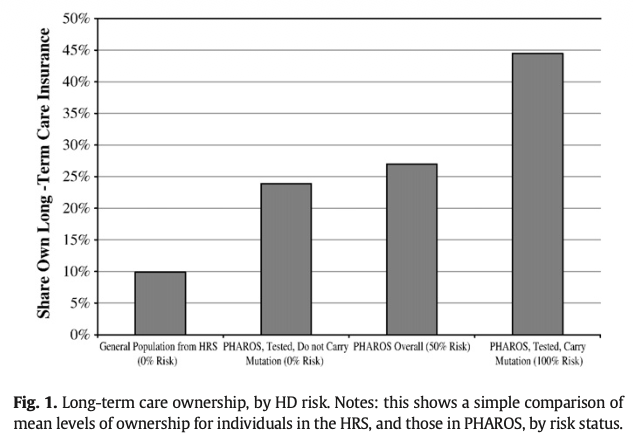
\includegraphics[width=0.7\textwidth]{./input/OSQD2010_fig1.png} 
\end{center}
\end{frame}
%---------------------------------------------------------------------
\begin{frame}{Huntington disease and adverse selection into LTC insurance}

    Oster, Shoulson, Quaid, Dorsey (2010) find \newbold{strong evidence of adverse selection}\\
    $\implies$ People who tested positive for the HD gene are \newbold{5$\times$ more likely} to buy LTC insurance\\
    \vspace{5mm}

    Can you guess how the LTC insurance market has evolved since 2010?\\
    \pause
    % That's a market that has decreased in size a lot with a lot of exit: adverse selection, Medicaid crowd out, insurers underestimated longevity and had to hike up premiums a lot
    \vspace{10mm}

    What about health insurance in general?\\
    \pause
    $\implies$ Let's look at the impact of \newbold{a mandate}.

    
\end{frame}
%---------------------------------------------------------------------
\begin{frame}{Mandates: Hackmann, Kolstad, Kowalski (2015)}
\begin{center}
    \only<1>{
\includegraphics[width=0.75\textwidth]{./input/HKK2015_front.png}   }
    \only<2>{
\includegraphics[width=0.75\textwidth]{./input/HKK2015_front2.png}   } 
\end{center}
\end{frame}
%---------------------------------------------------------------------
\begin{frame}{Massachussetts Health Reform (2006)}

    Mandate
    \vspace{-38mm}
    \begin{center}
        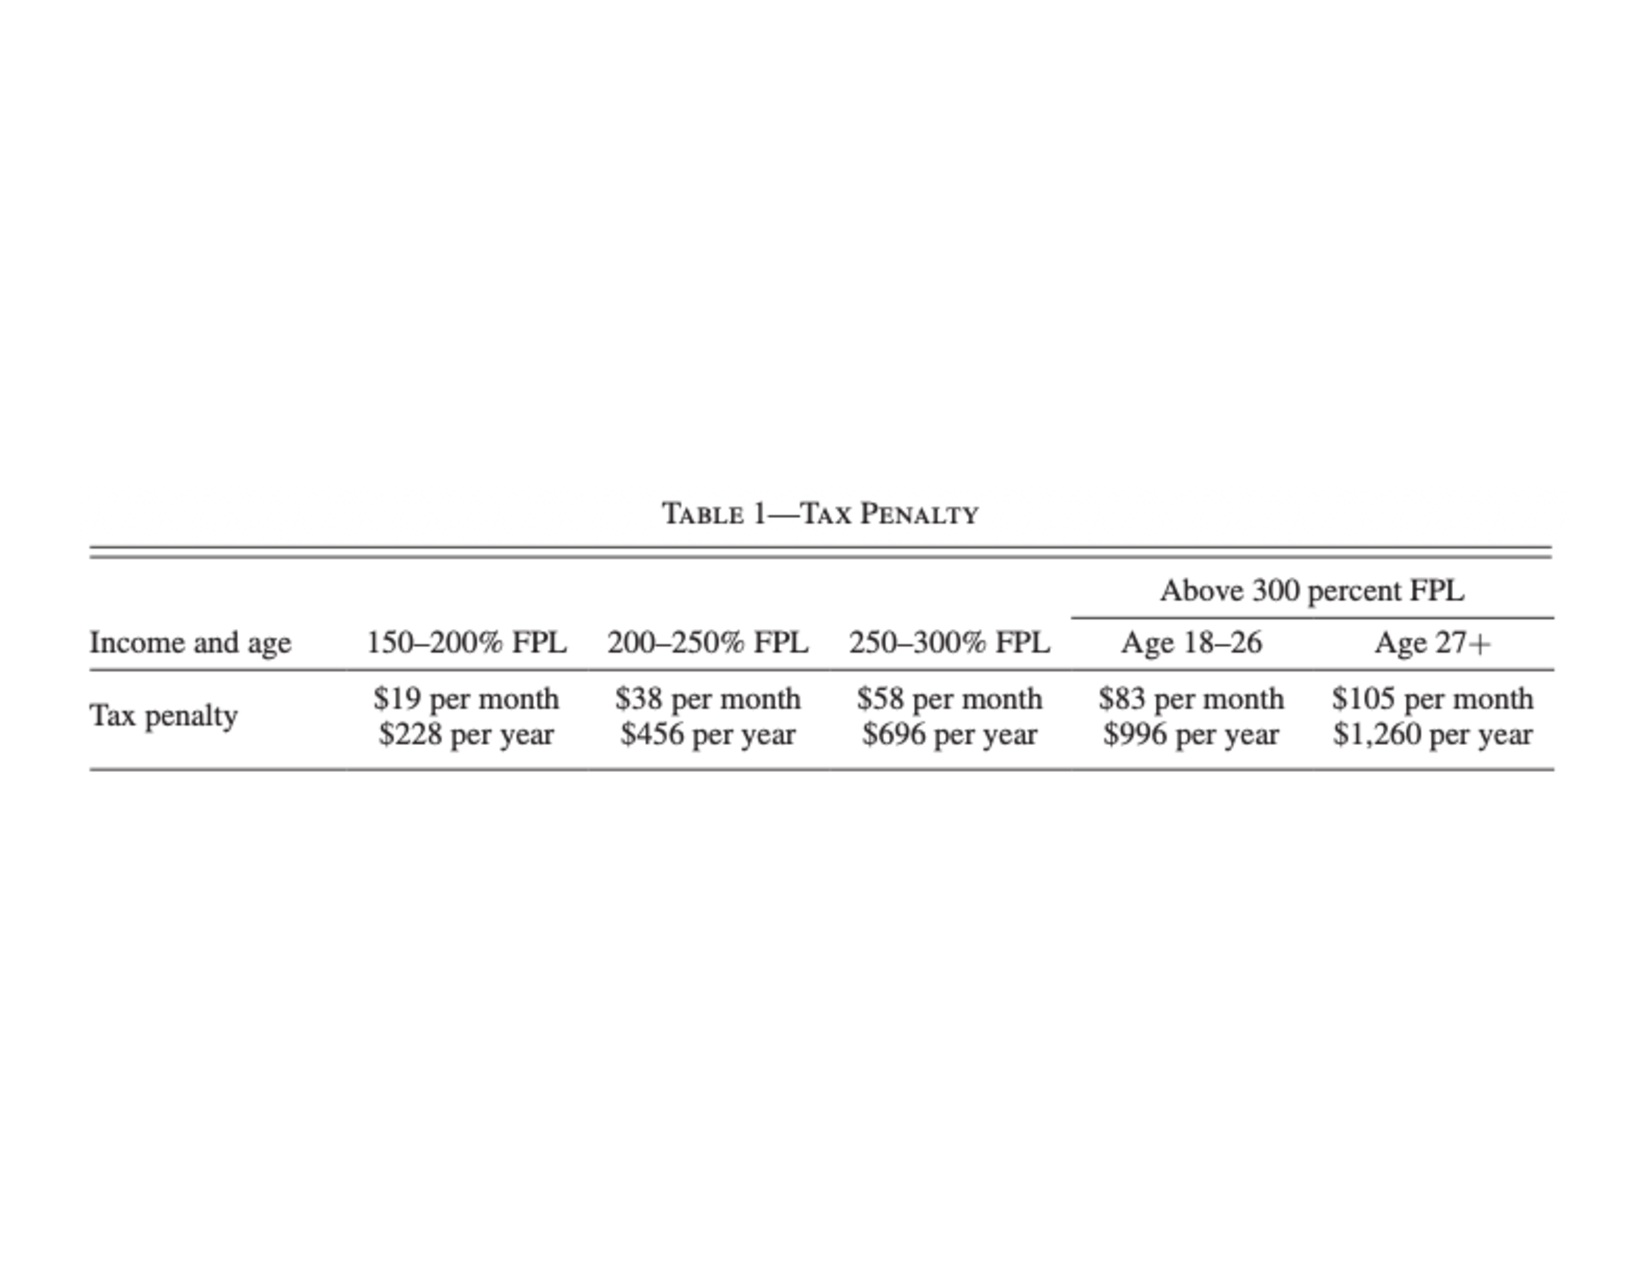
\includegraphics[width=0.9\textwidth]{./input/HKK2015_tab1.pdf}
    \end{center}
    \vspace{-38mm}
    \pause

    Who will be mostly impacted? People buying insurance by themselves (``non-group'')\\
    \vspace{2mm}
    \pause

    Two things that could exacerbate adverse selection in MA
    \begin{itemize}
        \item Community ratings: same price for people with same age
        \item Guaranteed issue (since 1996): cannot deny coverage for insurers with 5,000+ members
    \end{itemize}
    
    
\end{frame}
%---------------------------------------------------------------------
\begin{frame}{Mandates in theory}

\begin{center}
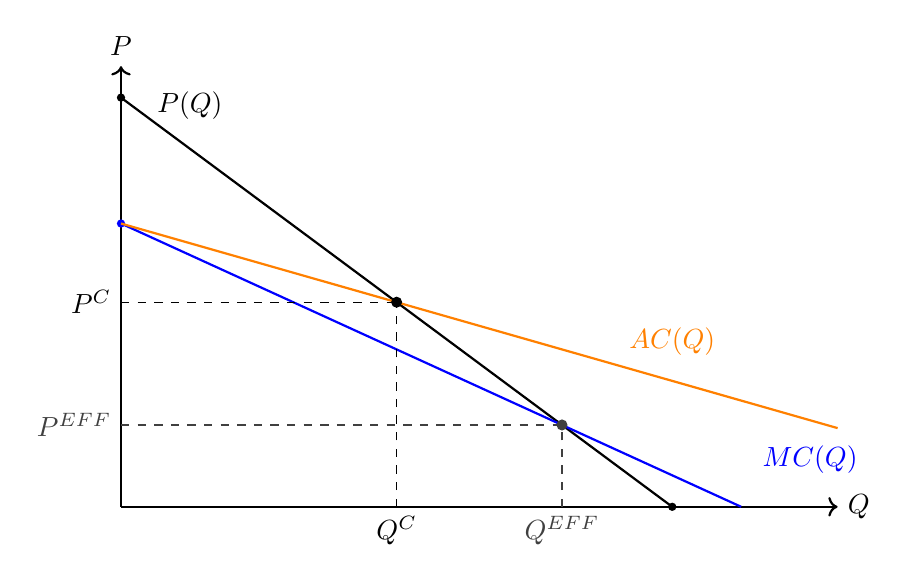
\begin{tikzpicture}[x=0.035cm, y=0.0020cm, scale=0.5]
\usetikzlibrary{arrows.meta}

    % Axes
    \draw[->, thick] (0,0) -- (520,0) node[right] {$Q$};
    \draw[->, thick] (0,0) -- (0,5600) node[above] {$P$};

    % Demand curve: P(Q) = 5200 - 13Q
    \draw[thick] (0,5200) -- (400,0);
    \node at (50,5100) {$P(Q)$};

    % Demand intercepts
    \fill (0,5200) circle[radius=3pt];
    \node[left] at (0,5200) {};

    \fill (400,0) circle[radius=3pt];
    \node[below] at (400,0) {};

    % ---- Marginal cost (lowered, same slope) ----
    % MC(Q) = 3600 - 8Q (x-intercept at Q=450)
    \draw[blue, thick] (0,3600) -- (450,0);
    \node[blue] at (500,600) {$MC(Q)$};

    \fill[blue] (0,3600) circle[radius=3pt];
    \node[left, blue] at (0,3600) {};

    % Average cost curve (lowered, same slope): AC(Q) = 3600 - 5Q
    \draw[orange, thick] (0,3600) -- (520,1000);
    \node[orange] at (400,2100) {$AC(Q)$};

    % Perfect competition equilibrium: intersection of Demand and AC
    % Solve: 5200-13Q = 3600-5Q  => 1600 = 8Q => Q=200, P=2600
    \fill (200,2600) circle[radius=4pt];
    \draw[dashed] (200,0) -- (200,2600);
    \draw[dashed] (0,2600) -- (200,2600);

    \node[below] at (200,0) {$Q^{C}$};
    \node[left] at (0,2600) {$P^{C}$};

    % ---- Efficient equilibrium: intersection of Demand and MC ----
    % Solve: 5200-13Q = 3600-8Q  => 1600 = 5Q => Q=320, P=1040
    \fill[darkgray] (320,1040) circle[radius=4pt];
    \draw[dashed, darkgray] (320,0) -- (320,1040);
    \draw[dashed, darkgray] (0,1040) -- (320,1040);

    \node[below, darkgray] at (320,0) {$Q^{EFF}$};
    \node[left,  darkgray] at (0,1040) {$P^{EFF}$};

\end{tikzpicture}
\end{center}
    %Note, may be targetted (low versus high income. Think of the line for one income)
    
    
\end{frame}
%---------------------------------------------------------------------
\begin{frame}{Mandates in theory}

\begin{center}
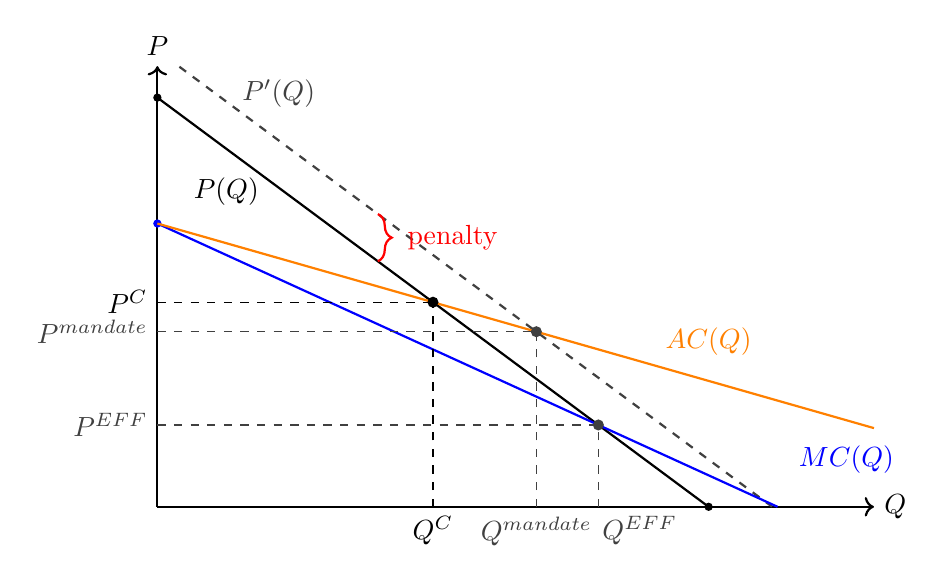
\begin{tikzpicture}[x=0.035cm, y=0.0020cm, scale=0.5]
\usetikzlibrary{arrows.meta}

    % Axes
    \draw[->, thick] (0,0) -- (520,0) node[right] {$Q$};
    \draw[->, thick] (0,0) -- (0,5600) node[above] {$P$};

    % Demand curve: P(Q) = 5200 - 13Q
    \draw[thick] (0,5200) -- (400,0);
    \node at (50,4000) {$P(Q)$};

    % New demand with mandate/penalty: P'(Q) = 5800 - 13Q
    \draw[darkgray, dashed, thick] (16,5592) -- (446,2);
    \node[darkgray] at (88,5250) {$P'(Q)$};

    % Demand intercepts
    \fill (0,5200) circle[radius=3pt];
    \node[left] at (0,5200) {};

    \fill (400,0) circle[radius=3pt];
    \node[below] at (400,0) {};

    % ---- Marginal cost (lowered, same slope) ----
    % MC(Q) = 3600 - 8Q (x-intercept at Q=450)
    \draw[blue, thick] (0,3600) -- (450,0);
    \node[blue] at (500,600) {$MC(Q)$};

    \fill[blue] (0,3600) circle[radius=3pt];
    \node[left, blue] at (0,3600) {};

    % Average cost curve (lowered, same slope): AC(Q) = 3600 - 5Q
    \draw[orange, thick] (0,3600) -- (520,1000);
    \node[orange] at (400,2100) {$AC(Q)$};

    % Perfect competition equilibrium: intersection of Demand and AC
    % Solve: 5200-13Q = 3600-5Q  => 1600 = 8Q => Q=200, P=2600
    \fill (200,2600) circle[radius=4pt];
    \draw[dashed] (200,0) -- (200,2600);
    \draw[dashed] (0,2600) -- (200,2600);

    \node[below] at (200,0) {$Q^{C}$};
    \node[left] at (0,2600) {$P^{C}$};

    % Efficient equilibrium: intersection of Demand and MC
    % Solve: 5200-13Q = 3600-8Q  => 1600 = 5Q => Q=320, P=1040
    \fill[darkgray] (320,1040) circle[radius=4pt];
    \draw[dashed, darkgray] (320,0) -- (320,1040);
    \draw[dashed, darkgray] (0,1040) -- (320,1040);

    \node[below, darkgray] at (350,0) {$Q^{EFF}$};
    \node[left,  darkgray] at (0,1040) {$P^{EFF}$};

    % Mandate intersection: P'(Q) with AC
    % Solve: 5800-13Q = 3600-5Q  => 2200 = 8Q => Q=275, P=2225
    \fill[darkgray] (275,2225) circle[radius=4pt];
    \draw[dashed, darkgray] (275,0) -- (275,2225);
    \draw[dashed, darkgray] (0,2225) -- (275,2225);

    \node[below, darkgray] at (275,0) {$Q^{mandate}$};
    \node[left, darkgray] at (0,2225) {$P^{mandate}$};

    % Penalty wedge between demand curves (higher up the curves)
    \draw[red, decorate, decoration={brace,mirror,amplitude=5pt}, thick]
        (160,3120) -- (160,3720)
        node[midway, right=7pt, red] {penalty};

\end{tikzpicture}
\end{center}

\end{frame}
%---------------------------------------------------------------------
\begin{frame}{Mandate in theory, summary}

\begin{columns}[T,onlytextwidth]
\begin{column}{0.60\textwidth}
\hspace*{-6mm}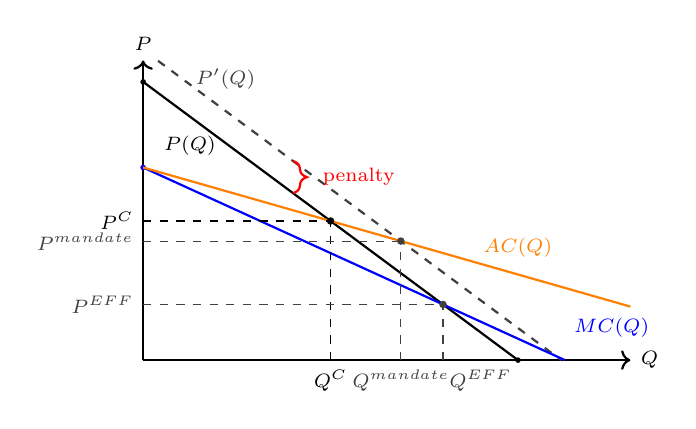
\begin{tikzpicture}[x=0.035cm, y=0.0020cm, scale=0.34, every node/.style={font=\scriptsize}]
\usetikzlibrary{arrows.meta}

    % Axes
    \draw[->, thick] (0,0) -- (520,0) node[right] {$Q$};
    \draw[->, thick] (0,0) -- (0,5600) node[above] {$P$};

    % Demand curve: P(Q) = 5200 - 13Q
    \draw[thick] (0,5200) -- (400,0);
    \node at (50,4000) {$P(Q)$};

    % New demand with mandate/penalty: P'(Q) = 5800 - 13Q
    \draw[darkgray, dashed, thick] (16,5592) -- (446,2);
    \node[darkgray] at (88,5250) {$P'(Q)$};

    % Demand intercepts
    \fill (0,5200) circle[radius=3pt];
    \node[left] at (0,5200) {};

    \fill (400,0) circle[radius=3pt];
    \node[below] at (400,0) {};

    % ---- Marginal cost (lowered, same slope) ----
    % MC(Q) = 3600 - 8Q (x-intercept at Q=450)
    \draw[blue, thick] (0,3600) -- (450,0);
    \node[blue] at (500,600) {$MC(Q)$};

    \fill[blue] (0,3600) circle[radius=3pt];
    \node[left, blue] at (0,3600) {};

    % Average cost curve (lowered, same slope): AC(Q) = 3600 - 5Q
    \draw[orange, thick] (0,3600) -- (520,1000);
    \node[orange] at (400,2100) {$AC(Q)$};

    % Perfect competition equilibrium: intersection of Demand and AC
    % Solve: 5200-13Q = 3600-5Q  => 1600 = 8Q => Q=200, P=2600
    \fill (200,2600) circle[radius=4pt];
    \draw[dashed] (200,0) -- (200,2600);
    \draw[dashed] (0,2600) -- (200,2600);

    \node[below] at (200,0) {$Q^{C}$};
    \node[left] at (0,2600) {$P^{C}$};

    % Efficient equilibrium: intersection of Demand and MC
    % Solve: 5200-13Q = 3600-8Q  => 1600 = 5Q => Q=320, P=1040
    \fill[darkgray] (320,1040) circle[radius=4pt];
    \draw[dashed, darkgray] (320,0) -- (320,1040);
    \draw[dashed, darkgray] (0,1040) -- (320,1040);

    \node[below, darkgray] at (360,0) {$Q^{EFF}$};
    \node[left,  darkgray] at (0,1040) {$P^{EFF}$};

    % Mandate intersection: P'(Q) with AC
    % Solve: 5800-13Q = 3600-5Q  => 2200 = 8Q => Q=275, P=2225
    \fill[darkgray] (275,2225) circle[radius=4pt];
    \draw[dashed, darkgray] (275,0) -- (275,2225);
    \draw[dashed, darkgray] (0,2225) -- (275,2225);

    \node[below, darkgray] at (275,0) {$Q^{mandate}$};
    \node[left, darkgray] at (0,2210) {$P^{mandate}$};

    % Penalty wedge between demand curves (higher up the curves)
    \draw[red, decorate, decoration={brace,mirror,amplitude=5pt}, thick]
        (160,3120) -- (160,3720)
        node[midway, right=7pt, red] {penalty};

\end{tikzpicture}

\end{column}
\begin{column}{0.40\textwidth}

    \begin{itemize}
        \item {\color{red}Penalty}: shifts demand up: $P(Q) \rightarrow P'(Q)$
        \item More people will get insurance: $Q^{C} \rightarrow Q^{mandate}$
        \item Average costs will decrease: $P^{C} \rightarrow P^{mandate}$\\
        \newbold{Why?}
        \only<1>{\\
        \vspace{25mm}}
        \only<2>{\textbf{Because healthier people buy insurance $\rightarrow AC(Q^{mandate})$ is lower}}
    \end{itemize}

\end{column}
\end{columns}
    
\end{frame}
%---------------------------------------------------------------------
\begin{frame}{Empirical method: difference-in-differences}

    How to get the effect of the mandate? Compare
    \begin{enumerate}
        \item Massachussetts and other states
        \item Before and after the reform
    \end{enumerate}
    $\implies$ \newbold{Difference-in-differences (DiD)} approach\\
    \textit{Warning: there are assumptions in this approach (e.g. ``parallel trend'')}
    \vspace{-3mm}

    \only<1>{
        \begin{align*}
        Y_{st}
        = \gamma (MA \times After)_{st}
        + \rho_1 & (MA \times During)_{st}
        + \rho_2 MA_s\\
        &+ \rho_3 After_t
        + \rho_4 During_t
        + \rho_5
        + \varepsilon_{st}
    \end{align*}
    \vspace{20mm}
    
    }
    \only<2>{
    \begin{align*}
        {\color{gray}Y_{st}}
        = {\color{maroon}\gamma} {\color{gray}(MA \times After)_{st}}
        + {\color{maroon}\rho_1} & {\color{gray}(MA \times During)_{st}}
        + {\color{maroon}\rho_2} {\color{gray}MA_s}\\
        &+ {\color{maroon}\rho_3} {\color{gray}After_t}
        + {\color{maroon}\rho_4} {\color{gray}During_t}
        + {\color{maroon}\rho_5}
        + \varepsilon_{st}
    \end{align*}
    with
    \begin{itemize}
        \item {\color{gray} Data}
        \item {\color{maroon} Parameters to estimate}
    \end{itemize}   
    Outcomes $Y_{st}$: insurance coverage, premiums, average costs for insurers
    }  
    
\end{frame}
%---------------------------------------------------------------------
\begin{frame}{Impact of the reform - insurance coverage}
\vspace{-35mm}

    \begin{center}
        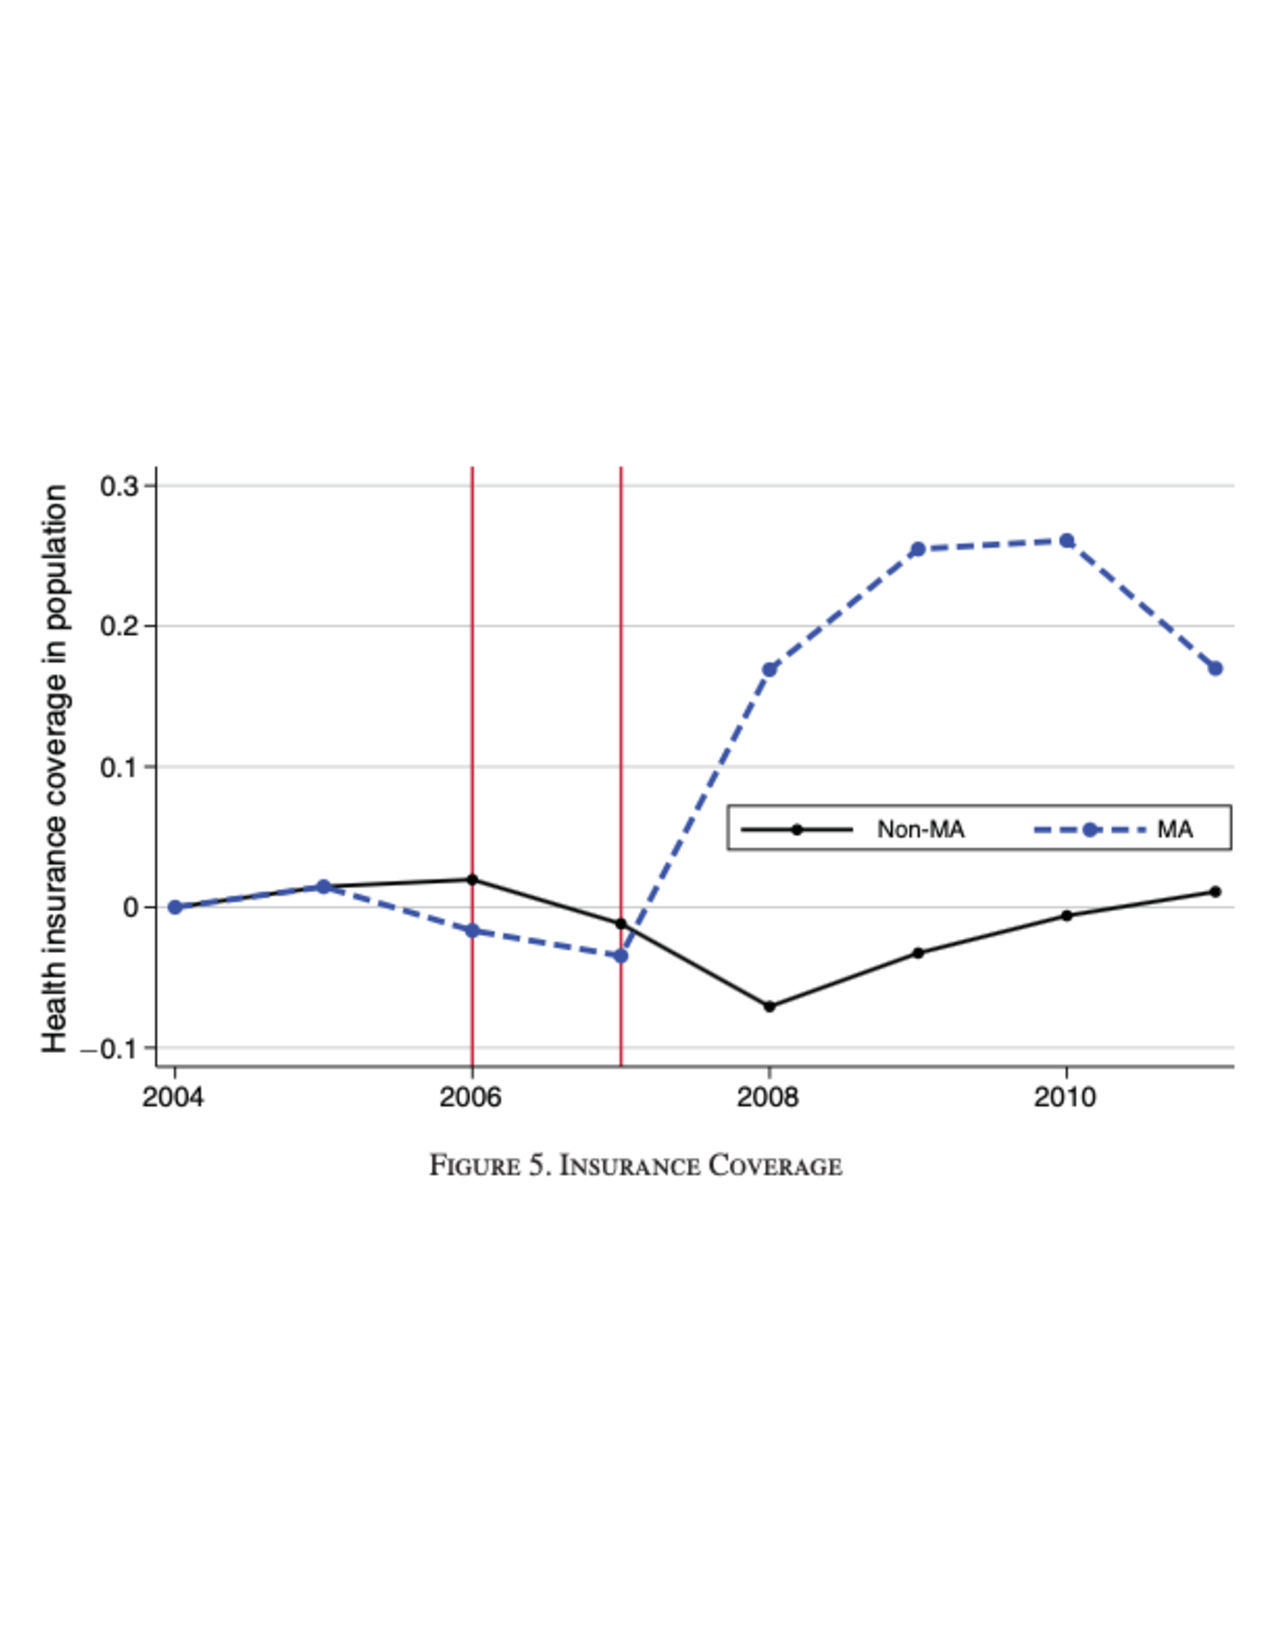
\includegraphics[width=0.8\textwidth]{./input/HKK2015_fig5.pdf}
    \end{center}    
    
\end{frame}
%---------------------------------------------------------------------
\begin{frame}{Impact of the reform - premium}
\vspace{-35mm}
    \begin{center}
        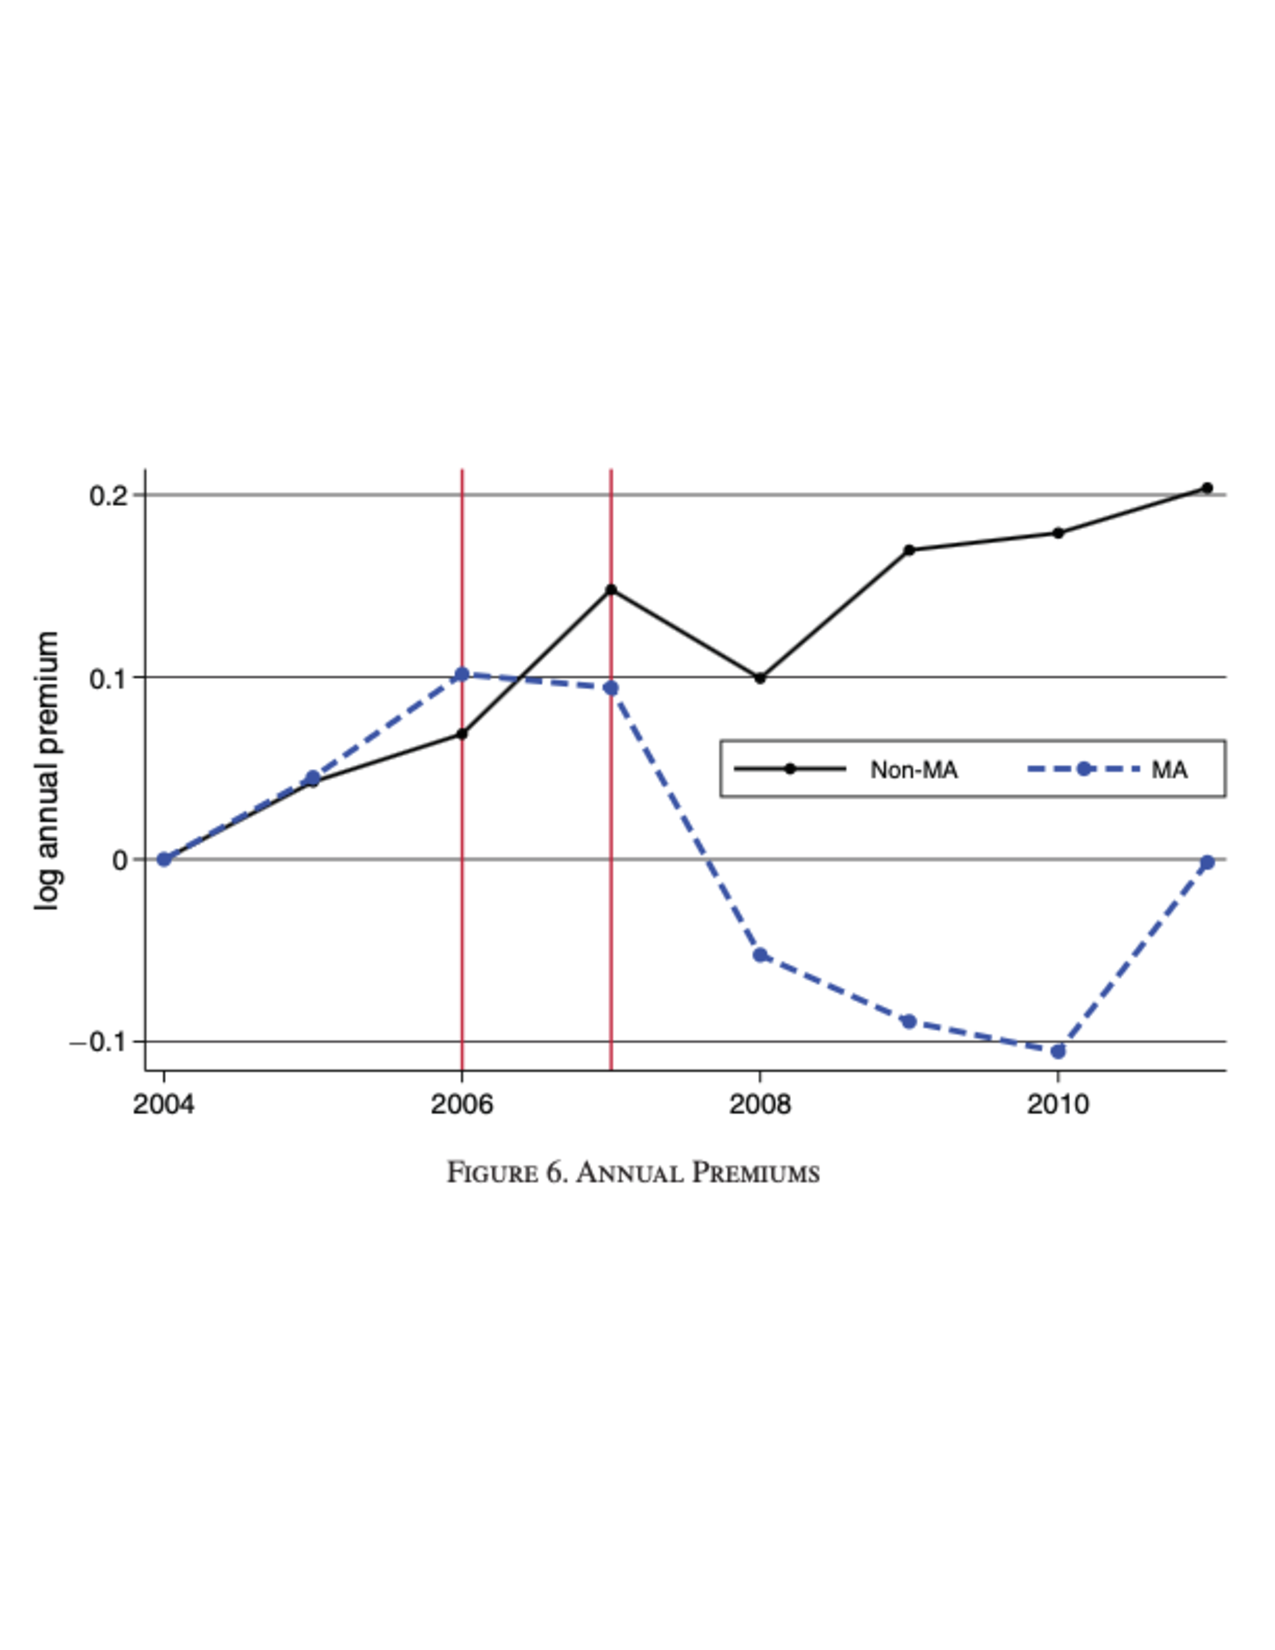
\includegraphics[width=0.8\textwidth]{./input/HKK2015_fig6.pdf}
    \end{center}    
    
\end{frame}
%---------------------------------------------------------------------
\begin{frame}{Impact of the reform - average costs}
\vspace{-35mm}

    \begin{center}
        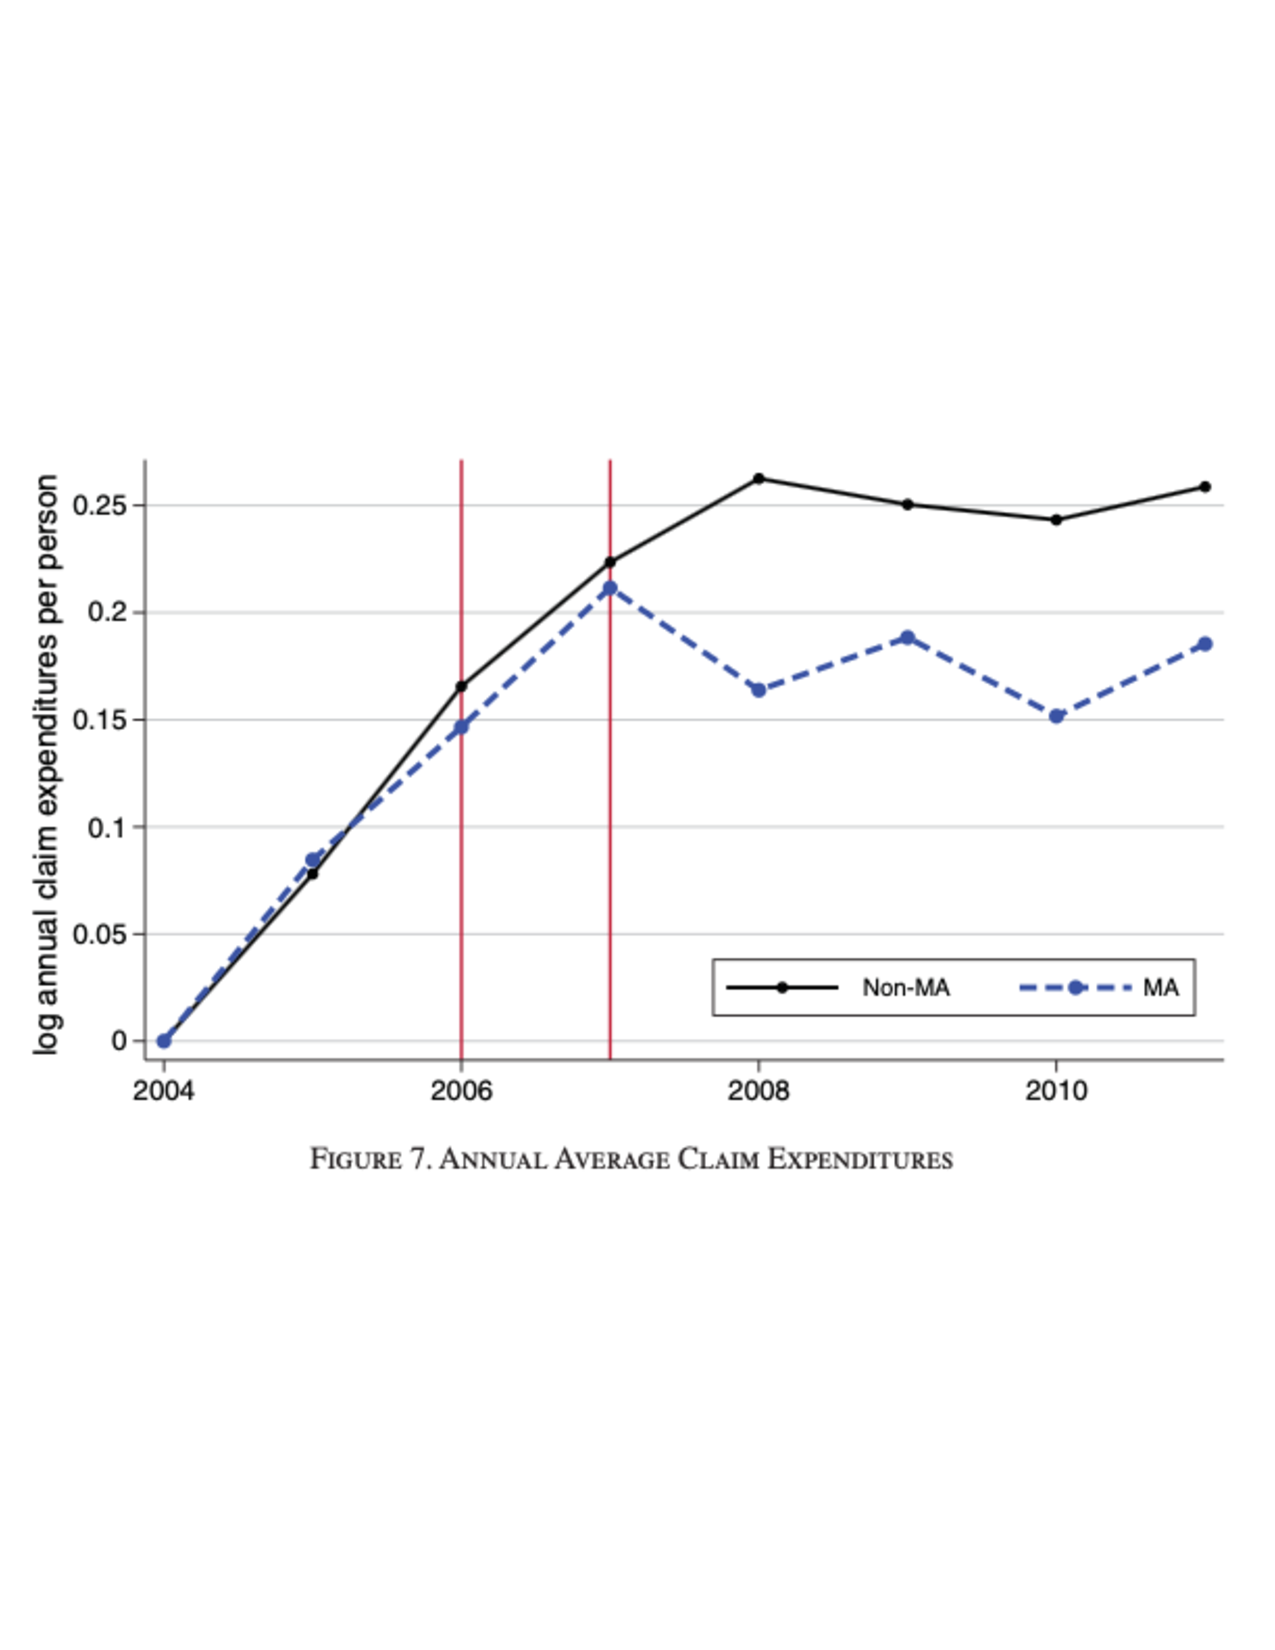
\includegraphics[width=0.8\textwidth]{./input/HKK2015_fig7.pdf}
    \end{center}    
    
\end{frame}
%---------------------------------------------------------------------
\begin{frame}{Summary}
    \vspace{-2mm}
    \begin{center}
        \only<1>{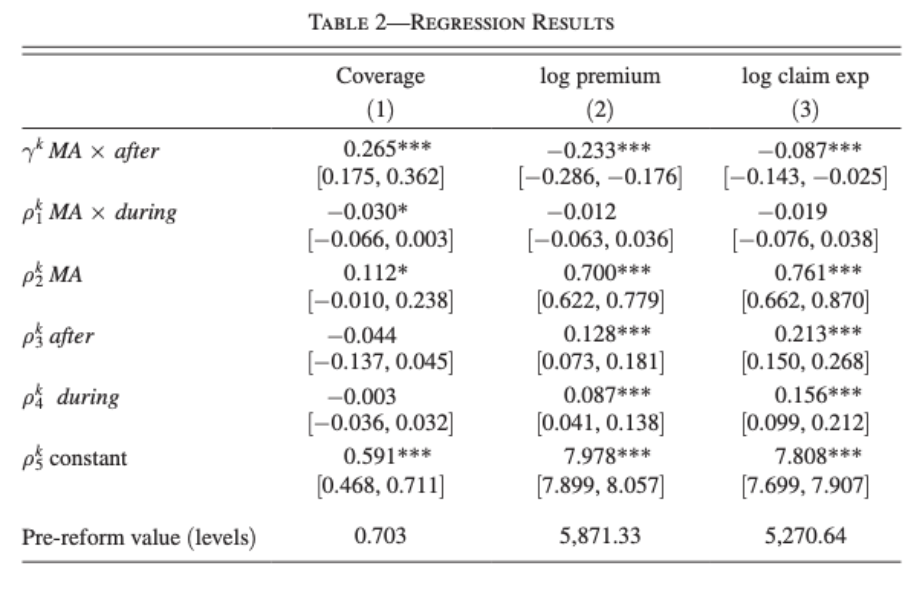
\includegraphics[width=0.88\textwidth]{./input/HKK2015_tab2.png}   }
        \only<2>{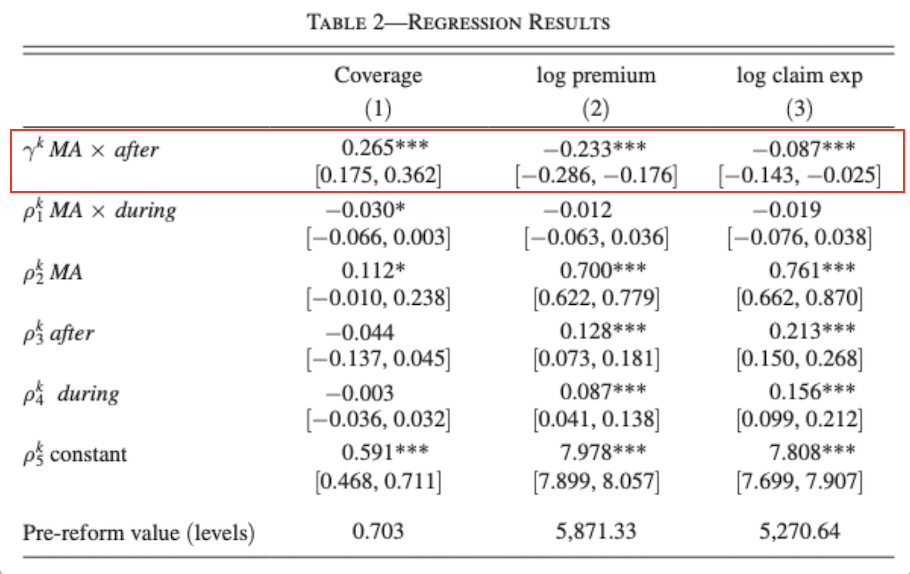
\includegraphics[width=0.88\textwidth]{./input/HKK2015_tab2H.png}   } 
    \end{center}    
    
\end{frame}
%---------------------------------------------------------------------
\begin{frame}{Hackmann, Kolstad, Kowalski (2015)}

    Why is this empirical evidence of adverse selection in Massachussetts?\\
    $\implies$ Average costs \newbold{decreased} with the mandate!

    \vspace{10mm}

    Thinking about implementing mandates:
    \begin{itemize}
        \item ``Stick'': penalty
        \item ``Carrot'': subsidies
    \end{itemize}
    
\end{frame}
%---------------------------------------------------------------------
\begin{frame}{Taking stock}

   There is evidence of adverse selection in the real world
    \begin{itemize}
         \item Huntington disease \& LTC insurance
         \item Massachussetts health reform \& the mandate
    \end{itemize}
    \vspace{5mm}

    Is the worst case scenario possible, i.e. full unraveling?
    
\end{frame}
%---------------------------------------------------------------------
\begin{frame}{Unraveling in theory}
\begin{center}
\only<1>{
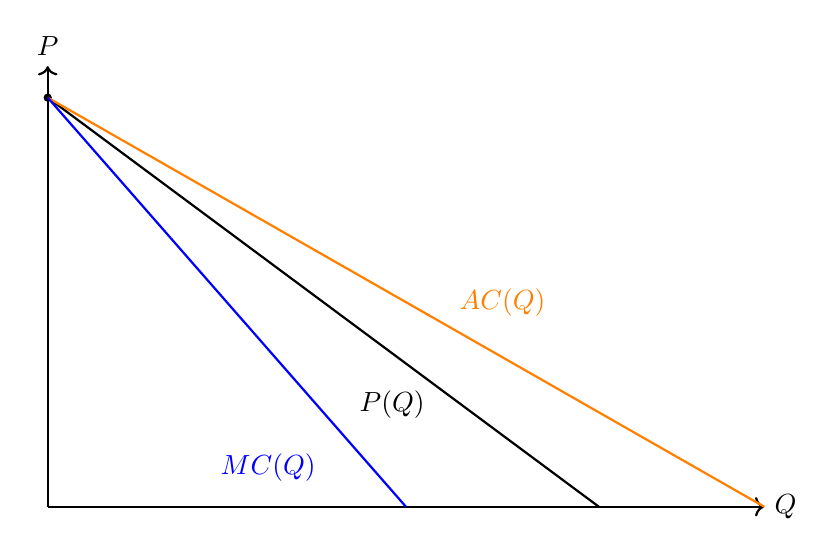
\begin{tikzpicture}[x=0.035cm, y=0.0020cm, scale=0.5]

    % Axes
    \draw[->, thick] (0,0) -- (520,0) node[right] {$Q$};
    \draw[->, thick] (0,0) -- (0,5600) node[above] {$P$};

    % Common intercept
    \fill (0,5200) circle[radius=3pt];

    % Demand curve: P(Q) = 5200 - 13Q
    \draw[thick] (0,5200) -- (400,0);
    \node at (250,1300) {$P(Q)$};

    % Average cost curve above demand: AC(Q) = 5200 - 10Q
    \draw[orange, thick] (0,5200) -- (520,0);
    \node[orange] at (330,2600) {$AC(Q)$};

    % Marginal cost curve below demand: MC(Q) = 5200 - 20Q
    \draw[blue, thick] (0,5200) -- (260,0);
    \node[blue] at (160,500) {$MC(Q)$};

\end{tikzpicture}
}
\only<2>{

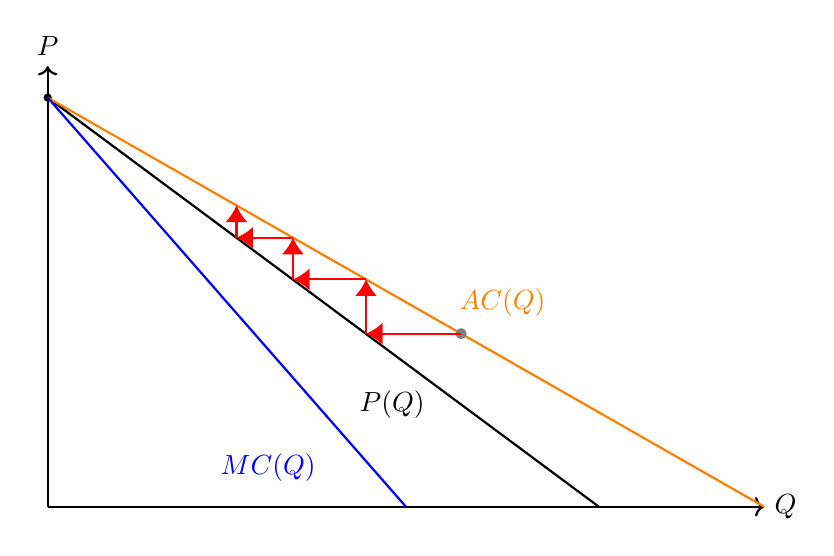
\begin{tikzpicture}[x=0.035cm, y=0.0020cm, scale=0.5]

    % Axes
    \draw[->, thick] (0,0) -- (520,0) node[right] {$Q$};
    \draw[->, thick] (0,0) -- (0,5600) node[above] {$P$};

    % Common intercept
    \fill (0,5200) circle[radius=3pt];

    % Demand curve: P(Q) = 5200 - 13Q
    \draw[thick] (0,5200) -- (400,0);
    \node at (250,1300) {$P(Q)$};

    % Average cost curve above demand: AC(Q) = 5200 - 10Q
    \draw[orange, thick] (0,5200) -- (520,0);
    \node[orange] at (330,2600) {$AC(Q)$};

    % Marginal cost curve below demand: MC(Q) = 5200 - 20Q
    \draw[blue, thick] (0,5200) -- (260,0);
    \node[blue] at (160,500) {$MC(Q)$};

    % Starting point on AC for the lowest arrow
    \fill[gray] (300,2200) circle[radius=4pt];

    % ---------- UNRAVELING STEPS (full arrow tips, 4 cycles) ----------

    % Left to demand
    \draw[-{Latex[length=6pt,width=8pt]}, thick, red] (300,2200) -- (231,2200);

    % Up to AC
    \draw[-{Latex[length=6pt,width=8pt]}, thick, red] (231,2200) -- (231,2890);

    % Left to demand
    \draw[-{Latex[length=6pt,width=8pt]}, thick, red] (231,2890) -- (178,2890);

    % Up to AC
    \draw[-{Latex[length=6pt,width=8pt]}, thick, red] (178,2890) -- (178,3420);

    % Left to demand  (NEW CYCLE)
    \draw[-{Latex[length=6pt,width=8pt]}, thick, red] (178,3420) -- (137,3420);

    % Up to AC  (NEW CYCLE)
    \draw[-{Latex[length=6pt,width=8pt]}, thick, red] (137,3420) -- (137,3830);

\end{tikzpicture}

}
\end{center}

\end{frame}
%---------------------------------------------------------------------
\begin{frame}{Unraveling in theory}
\usetikzlibrary{arrows.meta}
\begin{columns}[T,onlytextwidth]
\begin{column}{0.4\textwidth}
    \vspace{10mm}
\hspace*{-3mm}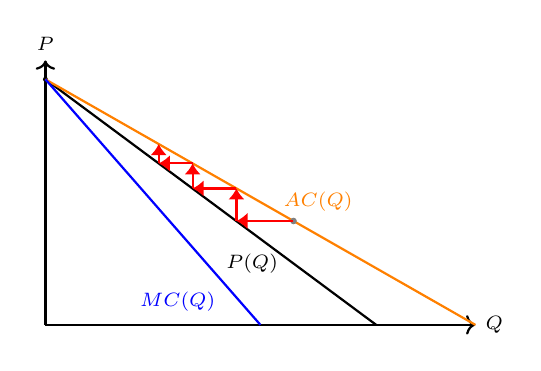
\begin{tikzpicture}[x=0.035cm, y=0.0020cm, scale=0.3, every node/.style={font=\scriptsize}]

    % Axes
    \draw[->, thick] (0,0) -- (520,0) node[right] {$Q$};
    \draw[->, thick] (0,0) -- (0,5600) node[above] {$P$};

    % Common intercept
    \fill (0,5200) circle[radius=3pt];

    % Demand curve: P(Q) = 5200 - 13Q
    \draw[thick] (0,5200) -- (400,0);
    \node at (250,1300) {$P(Q)$};

    % Average cost curve above demand: AC(Q) = 5200 - 10Q
    \draw[orange, thick] (0,5200) -- (520,0);
    \node[orange] at (330,2600) {$AC(Q)$};

    % Marginal cost curve below demand: MC(Q) = 5200 - 20Q
    \draw[blue, thick] (0,5200) -- (260,0);
    \node[blue] at (160,500) {$MC(Q)$};

    % Starting point on AC for the lowest arrow
    \fill[gray] (300,2200) circle[radius=4pt];

    % ---------- UNRAVELING STEPS (full arrow tips, 4 cycles) ----------

    % Left to demand
    \draw[-{Latex[length=4pt,width=6pt]}, thick, red] (300,2200) -- (231,2200);

    % Up to AC
    \draw[-{Latex[length=4pt,width=6pt]}, thick, red] (231,2200) -- (231,2890);

    % Left to demand
    \draw[-{Latex[length=4pt,width=6pt]}, thick, red] (231,2890) -- (178,2890);

    % Up to AC
    \draw[-{Latex[length=4pt,width=6pt]}, thick, red] (178,2890) -- (178,3420);

    % Left to demand  (NEW CYCLE)
    \draw[-{Latex[length=4pt,width=6pt]}, thick, red] (178,3420) -- (137,3420);

    % Up to AC  (NEW CYCLE)
    \draw[-{Latex[length=4pt,width=6pt]}, thick, red] (137,3420) -- (137,3830);

\end{tikzpicture}
\end{column}

\begin{column}{0.6\textwidth}
\begin{itemize}
    \item Some consumers would be willing to purchase insurance $MC(Q) < P(Q)$
    \item Start on gray point. Assume the insurer sets this premium.
    \item Healthier people drop the plan because too expensive ({\color{red}arrows} going to the left)
    \item At this premium, the insurer cannot cover its costs, so increases the premium to break even ({\color{red}arrows} going up)
\end{itemize}
\end{column}
\end{columns}
\end{frame}
%---------------------------------------------------------------------
\begin{frame}{The Harvard Death Spiral}

    References: \textit{Cutler and Reber, 1998; Cutler and Zeckhauser, 1998}\\
    \vspace{3mm}

    % Story of Sarah Reber for her thesis, interested in managed care (competition of plans within employer)
    % Idea: adverse selection so voucher is good but competition can lower premium. What to do? They find that competition lowers premiums.

    Two plans were offered by Harvard to its employees: PPO plan and HMO plan
    \begin{itemize}
        \item Harvard subsidized the PPO plan more than the HMO plan...
        \item ... but \newbold{in 1995}, stopped subsidizing the PPO plan more (budget tightening)
    \end{itemize}
    $\implies$ in 1995, the PPO plan started costing more for employees\\
    \vspace{3mm}

    What do you think happened?
    \only<1>{
        \\
        \vspace{20mm}
    }
    \only<2>{\begin{itemize}
        \item Price increase: less people enrolled in the PPO plan. Not surprising.
    \end{itemize}
    \vspace{10mm}}
    \only<3>{\begin{itemize}
        \item Price increase: less people enrolled in the PPO plan. Not surprising.
        \item What will happen to the price charged by insurers and why?
    \end{itemize}}
        \only<4>{\begin{itemize}
        \item Price increase: less people enrolled in the PPO plan. Not surprising.
        \item What will happen to the price charged by insurers and why?\\
        \newbold{Who} drops the PPO plan?
    \end{itemize}}
    
\end{frame}
%---------------------------------------------------------------------
\begin{frame}{The Harvard Death Spiral}

\begin{center}
    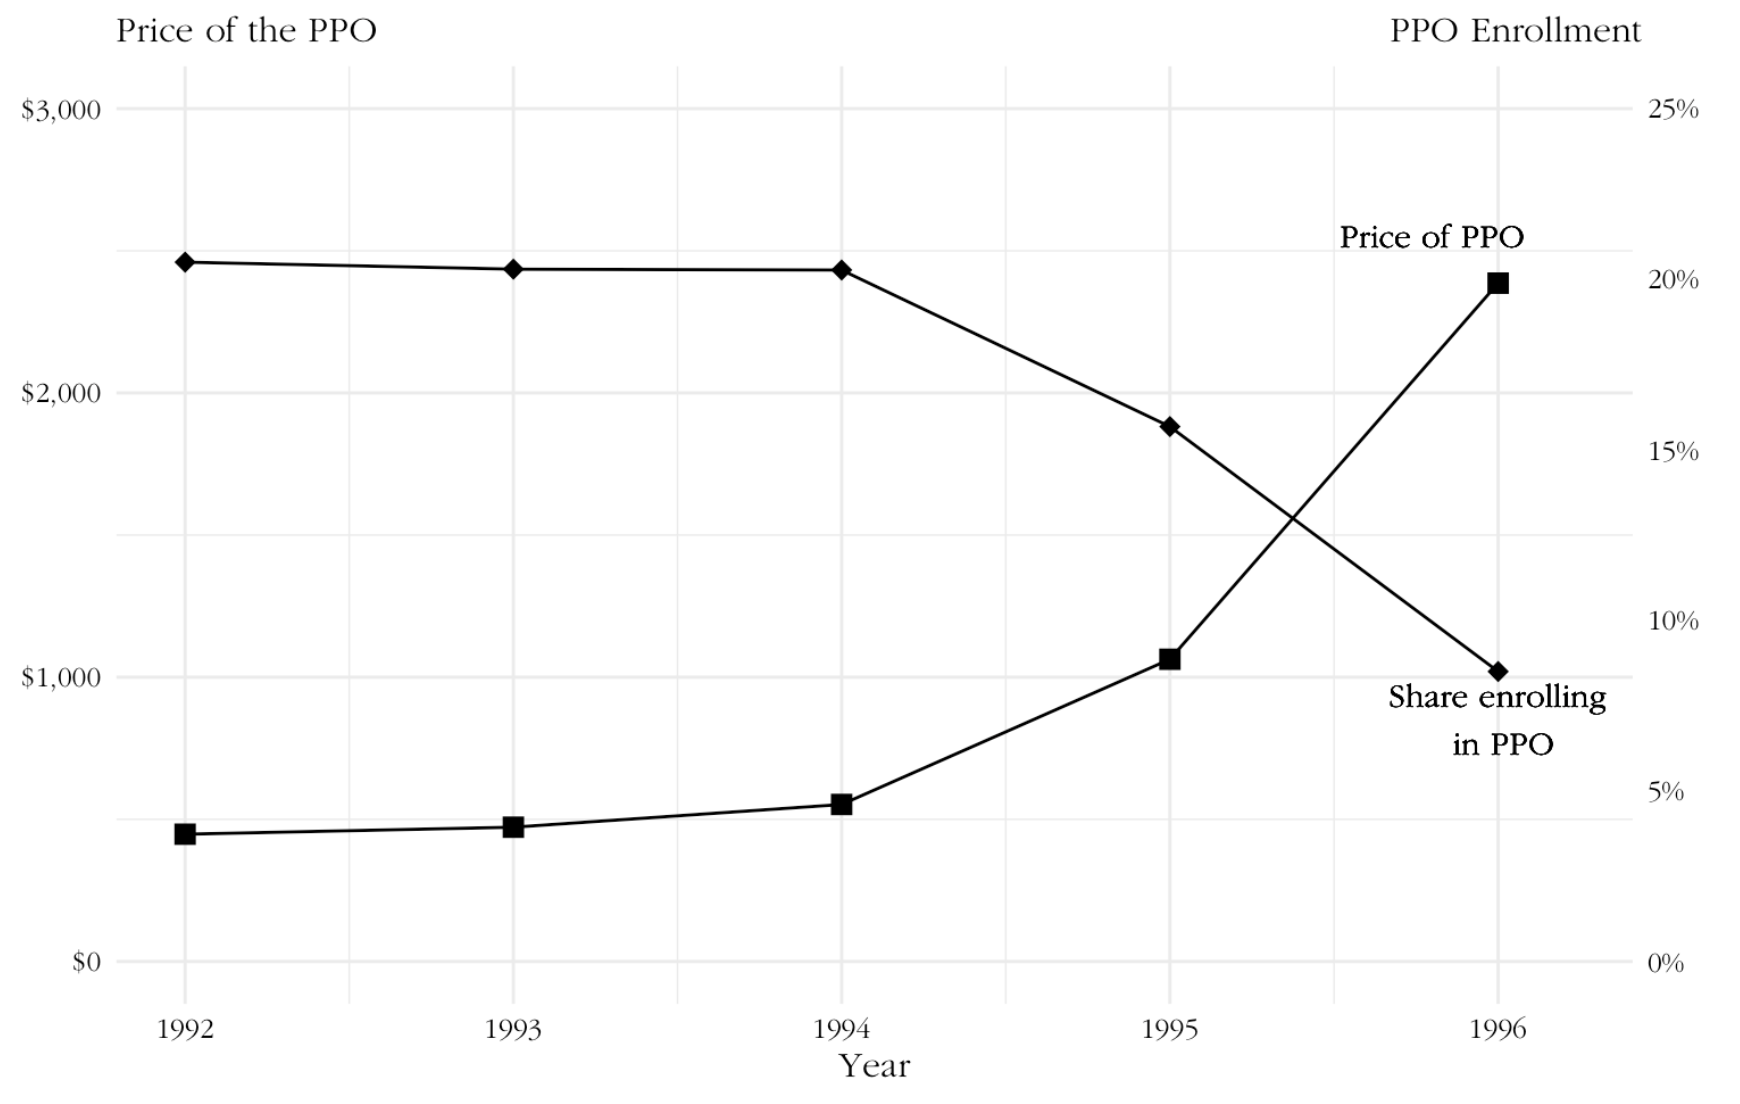
\includegraphics[width=0.8\textwidth]{./input/deathspiral_fig1.png}
\end{center}    
\end{frame}
%---------------------------------------------------------------------
\begin{frame}{The Harvard Death Spiral: conclusion}

    Harvard change in 1995: employees started paying more for the PPO plan
    \begin{itemize}
        \item Higher premium: less enrollment in the plan
        \item But also: premium charged by insurers to Harvard started increasing too!\\
        \newbold{Why?} Healthier employees dropped first $\rightarrow$ increase in average cost for insurers $\rightarrow$ increase in premium \\
        $\implies$ Real world \newbold{unraveling}
    \end{itemize}
    \vspace{5mm}

    Full unraveling: the PPO plan became too expensive to be sustainable and ended up terminated by Harvard
    
\end{frame}
%---------------------------------------------------------------------
\begin{frame}{Conclusion}

    Last class
    \begin{itemize}
        \item Saw how \newbold{asymmetric information} and \newbold{adverse selection} can lead to \textbf{market failure} in health insurance in theory\\
        \textit{Note: what does \textbf{market failure} mean here?}
    \end{itemize}
    \vspace{2mm}

    Today
    \begin{itemize}
        \item Confronted theory with reality: empirical evidence for
        \begin{itemize}
            \item Adverse selection {\small (Oster, Shoulson, Quaid, Dorsey, 2010; Hackmann, Kolstad, Kowalski, 2015)}
            \item Unraveling in the health insurance market {\small (Cutler and Reber, 1998; Cutler and Zeckhauser, 1998)}
        \end{itemize}
    \end{itemize}
    \vspace{2mm}

    What happens if health insurers manipulate contract features to attract/avoid certain types of consumers?
    \pause
    $\implies$ Next class: Rothschild-Stiglitz (1976)

    
\end{frame}
%---------------------------------------------------------------------
\begin{frame}{}
    \begin{center}
    \Large \textcolor{maroon}{Wrapping up}
    \end{center}
\end{frame}
%---------------------------------------------------------------------
\begin{frame}{To next class}
\begin{itemize}
    \item \newbold{TO DO}
    \begin{enumerate}
        \item \newbold{Problem set 3}: due next \newbold{Thursday, March 5 at 9:30am}
        \item Optional readings for next class:
        \begin{enumerate}
            \item Rothschild and Stiglitz (1976)
            \item Geruso and Layton (2017) \textit{``Selection in Insurance Markets and Its Policy Remedies''}
        \end{enumerate}
        \item Review this class and past material $\implies$ \textit{questions on it?}
    \end{enumerate}
    \vspace{5mm}

    \item Program for next class
    \begin{itemize}
        \item Allowing contract features beyond premium to adjust: Rothschild-Stiglitz (1976)
    \end{itemize}
\end{itemize}
\end{frame}
%---------------------------------------------------------------------
%---------------------------------------------------------------------

%%---------------------------------------------------------------------
% \appendix
% \setbeamertemplate{footline}{\hfill Appendix: \insertframenumber}
% \begin{frame}[plain] \begin{center}{\LARGE Appendix}\end{center} \end{frame}


\end{document}